% Created by tikzDevice version 0.12 on 2021-06-19 15:41:28
% !TEX encoding = UTF-8 Unicode
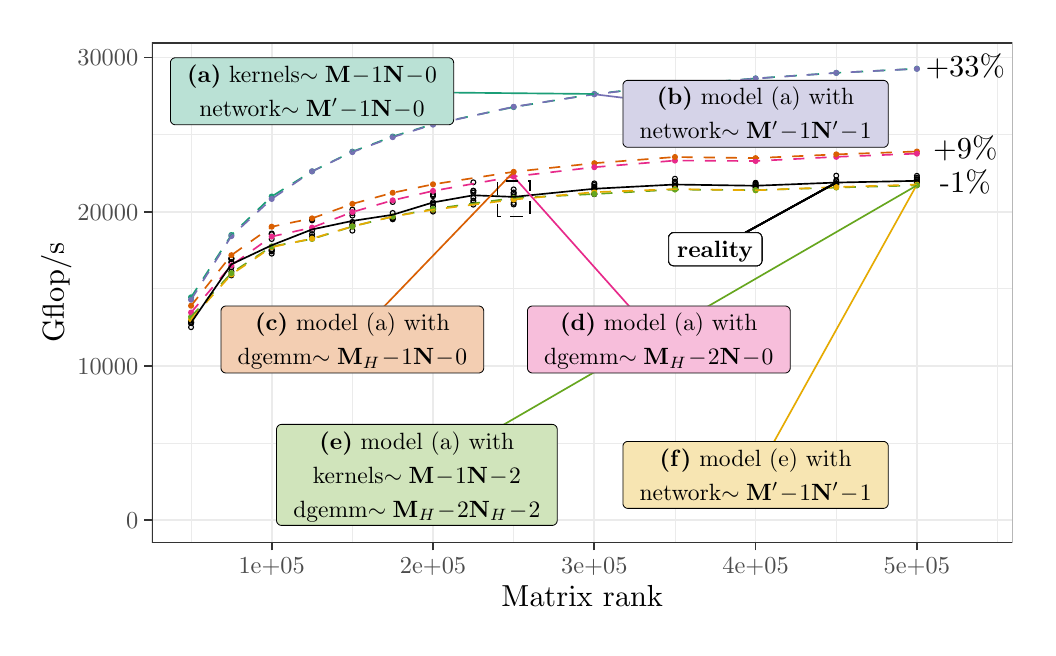
\begin{tikzpicture}[x=1pt,y=1pt]
\definecolor{fillColor}{RGB}{255,255,255}
\path[use as bounding box,fill=fillColor,fill opacity=0.00] (0,0) rectangle (361.35,216.81);
\begin{scope}
\path[clip] (  0.00,  0.00) rectangle (361.35,216.81);
\definecolor{drawColor}{RGB}{255,255,255}
\definecolor{fillColor}{RGB}{255,255,255}

\path[draw=drawColor,line width= 0.6pt,line join=round,line cap=round,fill=fillColor] (  0.00,  0.00) rectangle (361.35,216.81);
\end{scope}
\begin{scope}
\path[clip] ( 44.91, 30.69) rectangle (355.85,211.31);
\definecolor{fillColor}{RGB}{255,255,255}

\path[fill=fillColor] ( 44.91, 30.69) rectangle (355.85,211.31);
\definecolor{drawColor}{gray}{0.92}

\path[draw=drawColor,line width= 0.3pt,line join=round] ( 44.91, 66.75) --
	(355.85, 66.75);

\path[draw=drawColor,line width= 0.3pt,line join=round] ( 44.91,122.45) --
	(355.85,122.45);

\path[draw=drawColor,line width= 0.3pt,line join=round] ( 44.91,178.15) --
	(355.85,178.15);

\path[draw=drawColor,line width= 0.3pt,line join=round] ( 59.04, 30.69) --
	( 59.04,211.31);

\path[draw=drawColor,line width= 0.3pt,line join=round] (117.33, 30.69) --
	(117.33,211.31);

\path[draw=drawColor,line width= 0.3pt,line join=round] (175.61, 30.69) --
	(175.61,211.31);

\path[draw=drawColor,line width= 0.3pt,line join=round] (233.89, 30.69) --
	(233.89,211.31);

\path[draw=drawColor,line width= 0.3pt,line join=round] (292.18, 30.69) --
	(292.18,211.31);

\path[draw=drawColor,line width= 0.3pt,line join=round] (350.46, 30.69) --
	(350.46,211.31);

\path[draw=drawColor,line width= 0.6pt,line join=round] ( 44.91, 38.90) --
	(355.85, 38.90);

\path[draw=drawColor,line width= 0.6pt,line join=round] ( 44.91, 94.60) --
	(355.85, 94.60);

\path[draw=drawColor,line width= 0.6pt,line join=round] ( 44.91,150.30) --
	(355.85,150.30);

\path[draw=drawColor,line width= 0.6pt,line join=round] ( 44.91,206.00) --
	(355.85,206.00);

\path[draw=drawColor,line width= 0.6pt,line join=round] ( 88.18, 30.69) --
	( 88.18,211.31);

\path[draw=drawColor,line width= 0.6pt,line join=round] (146.47, 30.69) --
	(146.47,211.31);

\path[draw=drawColor,line width= 0.6pt,line join=round] (204.75, 30.69) --
	(204.75,211.31);

\path[draw=drawColor,line width= 0.6pt,line join=round] (263.03, 30.69) --
	(263.03,211.31);

\path[draw=drawColor,line width= 0.6pt,line join=round] (321.32, 30.69) --
	(321.32,211.31);
\definecolor{drawColor}{RGB}{0,0,0}

\path[draw=drawColor,line width= 0.4pt,line join=round,line cap=round] (321.32,163.27) circle (  0.89);

\path[draw=drawColor,line width= 0.4pt,line join=round,line cap=round] ( 59.04,110.08) circle (  0.89);

\path[draw=drawColor,line width= 0.4pt,line join=round,line cap=round] (204.75,156.65) circle (  0.89);

\path[draw=drawColor,line width= 0.4pt,line join=round,line cap=round] (263.03,159.54) circle (  0.89);

\path[draw=drawColor,line width= 0.4pt,line join=round,line cap=round] (117.33,149.79) circle (  0.89);

\path[draw=drawColor,line width= 0.4pt,line join=round,line cap=round] (175.61,153.47) circle (  0.89);

\path[draw=drawColor,line width= 0.4pt,line join=round,line cap=round] (292.18,161.66) circle (  0.89);

\path[draw=drawColor,line width= 0.4pt,line join=round,line cap=round] (233.89,162.22) circle (  0.89);

\path[draw=drawColor,line width= 0.4pt,line join=round,line cap=round] (146.47,153.75) circle (  0.89);

\path[draw=drawColor,line width= 0.4pt,line join=round,line cap=round] ( 88.18,142.16) circle (  0.89);

\path[draw=drawColor,line width= 0.4pt,line join=round,line cap=round] ( 73.61,133.53) circle (  0.89);

\path[draw=drawColor,line width= 0.4pt,line join=round,line cap=round] (102.76,147.18) circle (  0.89);

\path[draw=drawColor,line width= 0.4pt,line join=round,line cap=round] (161.04,157.93) circle (  0.89);

\path[draw=drawColor,line width= 0.4pt,line join=round,line cap=round] ( 73.61,133.36) circle (  0.89);

\path[draw=drawColor,line width= 0.4pt,line join=round,line cap=round] (204.75,160.54) circle (  0.89);

\path[draw=drawColor,line width= 0.4pt,line join=round,line cap=round] (292.18,163.33) circle (  0.89);

\path[draw=drawColor,line width= 0.4pt,line join=round,line cap=round] (146.47,156.59) circle (  0.89);

\path[draw=drawColor,line width= 0.4pt,line join=round,line cap=round] (131.90,147.73) circle (  0.89);

\path[draw=drawColor,line width= 0.4pt,line join=round,line cap=round] ( 59.04,110.14) circle (  0.89);

\path[draw=drawColor,line width= 0.4pt,line join=round,line cap=round] (161.04,160.93) circle (  0.89);

\path[draw=drawColor,line width= 0.4pt,line join=round,line cap=round] (175.61,157.26) circle (  0.89);

\path[draw=drawColor,line width= 0.4pt,line join=round,line cap=round] (102.76,140.94) circle (  0.89);

\path[draw=drawColor,line width= 0.4pt,line join=round,line cap=round] (117.33,146.62) circle (  0.89);

\path[draw=drawColor,line width= 0.4pt,line join=round,line cap=round] ( 88.18,142.44) circle (  0.89);

\path[draw=drawColor,line width= 0.4pt,line join=round,line cap=round] (321.32,162.05) circle (  0.89);

\path[draw=drawColor,line width= 0.4pt,line join=round,line cap=round] (263.03,160.77) circle (  0.89);

\path[draw=drawColor,line width= 0.4pt,line join=round,line cap=round] (233.89,158.71) circle (  0.89);

\path[draw=drawColor,line width= 0.4pt,line join=round,line cap=round] ( 59.04,110.41) circle (  0.89);

\path[draw=drawColor,line width= 0.4pt,line join=round,line cap=round] (102.76,140.77) circle (  0.89);

\path[draw=drawColor,line width= 0.4pt,line join=round,line cap=round] (321.32,160.21) circle (  0.89);

\path[draw=drawColor,line width= 0.4pt,line join=round,line cap=round] (161.04,153.69) circle (  0.89);

\path[draw=drawColor,line width= 0.4pt,line join=round,line cap=round] (117.33,148.90) circle (  0.89);

\path[draw=drawColor,line width= 0.4pt,line join=round,line cap=round] (263.03,159.99) circle (  0.89);

\path[draw=drawColor,line width= 0.4pt,line join=round,line cap=round] ( 73.61,128.68) circle (  0.89);

\path[draw=drawColor,line width= 0.4pt,line join=round,line cap=round] (204.75,158.43) circle (  0.89);

\path[draw=drawColor,line width= 0.4pt,line join=round,line cap=round] (233.89,160.27) circle (  0.89);

\path[draw=drawColor,line width= 0.4pt,line join=round,line cap=round] (292.18,161.27) circle (  0.89);

\path[draw=drawColor,line width= 0.4pt,line join=round,line cap=round] (175.61,154.59) circle (  0.89);

\path[draw=drawColor,line width= 0.4pt,line join=round,line cap=round] (146.47,155.92) circle (  0.89);

\path[draw=drawColor,line width= 0.4pt,line join=round,line cap=round] ( 88.18,135.98) circle (  0.89);

\path[draw=drawColor,line width= 0.4pt,line join=round,line cap=round] (131.90,148.01) circle (  0.89);

\path[draw=drawColor,line width= 0.4pt,line join=round,line cap=round] (175.61,156.31) circle (  0.89);

\path[draw=drawColor,line width= 0.4pt,line join=round,line cap=round] ( 59.04,108.58) circle (  0.89);

\path[draw=drawColor,line width= 0.4pt,line join=round,line cap=round] (204.75,158.37) circle (  0.89);

\path[draw=drawColor,line width= 0.4pt,line join=round,line cap=round] (102.76,141.27) circle (  0.89);

\path[draw=drawColor,line width= 0.4pt,line join=round,line cap=round] ( 88.18,136.71) circle (  0.89);

\path[draw=drawColor,line width= 0.4pt,line join=round,line cap=round] (321.32,162.61) circle (  0.89);

\path[draw=drawColor,line width= 0.4pt,line join=round,line cap=round] ( 73.61,132.14) circle (  0.89);

\path[draw=drawColor,line width= 0.4pt,line join=round,line cap=round] (117.33,145.23) circle (  0.89);

\path[draw=drawColor,line width= 0.4pt,line join=round,line cap=round] (146.47,153.25) circle (  0.89);

\path[draw=drawColor,line width= 0.4pt,line join=round,line cap=round] (263.03,159.99) circle (  0.89);

\path[draw=drawColor,line width= 0.4pt,line join=round,line cap=round] (161.04,155.31) circle (  0.89);

\path[draw=drawColor,line width= 0.4pt,line join=round,line cap=round] (292.18,159.38) circle (  0.89);

\path[draw=drawColor,line width= 0.4pt,line join=round,line cap=round] (131.90,148.24) circle (  0.89);

\path[draw=drawColor,line width= 0.4pt,line join=round,line cap=round] (233.89,159.65) circle (  0.89);

\path[draw=drawColor,line width= 0.4pt,line join=round,line cap=round] (146.47,150.85) circle (  0.89);

\path[draw=drawColor,line width= 0.4pt,line join=round,line cap=round] (292.18,160.21) circle (  0.89);

\path[draw=drawColor,line width= 0.4pt,line join=round,line cap=round] (131.90,149.85) circle (  0.89);

\path[draw=drawColor,line width= 0.4pt,line join=round,line cap=round] (263.03,158.43) circle (  0.89);

\path[draw=drawColor,line width= 0.4pt,line join=round,line cap=round] (175.61,155.42) circle (  0.89);

\path[draw=drawColor,line width= 0.4pt,line join=round,line cap=round] ( 59.04,111.08) circle (  0.89);

\path[draw=drawColor,line width= 0.4pt,line join=round,line cap=round] (204.75,158.82) circle (  0.89);

\path[draw=drawColor,line width= 0.4pt,line join=round,line cap=round] (321.32,159.88) circle (  0.89);

\path[draw=drawColor,line width= 0.4pt,line join=round,line cap=round] ( 73.61,133.14) circle (  0.89);

\path[draw=drawColor,line width= 0.4pt,line join=round,line cap=round] (102.76,147.62) circle (  0.89);

\path[draw=drawColor,line width= 0.4pt,line join=round,line cap=round] (117.33,151.08) circle (  0.89);

\path[draw=drawColor,line width= 0.4pt,line join=round,line cap=round] ( 88.18,135.15) circle (  0.89);

\path[draw=drawColor,line width= 0.4pt,line join=round,line cap=round] (161.04,154.31) circle (  0.89);

\path[draw=drawColor,line width= 0.4pt,line join=round,line cap=round] (233.89,158.54) circle (  0.89);

\path[draw=drawColor,line width= 0.4pt,line join=round,line cap=round] (321.32,160.77) circle (  0.89);

\path[draw=drawColor,line width= 0.4pt,line join=round,line cap=round] ( 59.04,110.19) circle (  0.89);

\path[draw=drawColor,line width= 0.4pt,line join=round,line cap=round] (204.75,156.70) circle (  0.89);

\path[draw=drawColor,line width= 0.4pt,line join=round,line cap=round] (263.03,159.32) circle (  0.89);

\path[draw=drawColor,line width= 0.4pt,line join=round,line cap=round] (117.33,145.73) circle (  0.89);

\path[draw=drawColor,line width= 0.4pt,line join=round,line cap=round] (175.61,156.98) circle (  0.89);

\path[draw=drawColor,line width= 0.4pt,line join=round,line cap=round] (292.18,160.27) circle (  0.89);

\path[draw=drawColor,line width= 0.4pt,line join=round,line cap=round] (233.89,159.54) circle (  0.89);

\path[draw=drawColor,line width= 0.4pt,line join=round,line cap=round] (146.47,150.35) circle (  0.89);

\path[draw=drawColor,line width= 0.4pt,line join=round,line cap=round] ( 88.18,136.26) circle (  0.89);

\path[draw=drawColor,line width= 0.4pt,line join=round,line cap=round] ( 73.61,130.24) circle (  0.89);

\path[draw=drawColor,line width= 0.4pt,line join=round,line cap=round] (102.76,147.68) circle (  0.89);

\path[draw=drawColor,line width= 0.4pt,line join=round,line cap=round] (161.04,157.15) circle (  0.89);

\path[draw=drawColor,line width= 0.4pt,line join=round,line cap=round] ( 73.61,127.29) circle (  0.89);

\path[draw=drawColor,line width= 0.4pt,line join=round,line cap=round] (204.75,159.99) circle (  0.89);

\path[draw=drawColor,line width= 0.4pt,line join=round,line cap=round] (292.18,159.99) circle (  0.89);

\path[draw=drawColor,line width= 0.4pt,line join=round,line cap=round] (146.47,152.19) circle (  0.89);

\path[draw=drawColor,line width= 0.4pt,line join=round,line cap=round] (131.90,153.81) circle (  0.89);

\path[draw=drawColor,line width= 0.4pt,line join=round,line cap=round] ( 59.04,110.41) circle (  0.89);

\path[draw=drawColor,line width= 0.4pt,line join=round,line cap=round] (161.04,152.86) circle (  0.89);

\path[draw=drawColor,line width= 0.4pt,line join=round,line cap=round] (175.61,152.91) circle (  0.89);

\path[draw=drawColor,line width= 0.4pt,line join=round,line cap=round] (102.76,143.50) circle (  0.89);

\path[draw=drawColor,line width= 0.4pt,line join=round,line cap=round] (117.33,143.45) circle (  0.89);

\path[draw=drawColor,line width= 0.4pt,line join=round,line cap=round] ( 88.18,136.37) circle (  0.89);

\path[draw=drawColor,line width= 0.4pt,line join=round,line cap=round] (321.32,161.05) circle (  0.89);

\path[draw=drawColor,line width= 0.4pt,line join=round,line cap=round] (263.03,160.43) circle (  0.89);

\path[draw=drawColor,line width= 0.4pt,line join=round,line cap=round] (233.89,160.88) circle (  0.89);

\path[draw=drawColor,line width= 0.4pt,line join=round,line cap=round] ( 59.04,110.53) circle (  0.89);

\path[draw=drawColor,line width= 0.4pt,line join=round,line cap=round] (102.76,142.22) circle (  0.89);

\path[draw=drawColor,line width= 0.4pt,line join=round,line cap=round] (321.32,161.83) circle (  0.89);

\path[draw=drawColor,line width= 0.4pt,line join=round,line cap=round] (161.04,157.76) circle (  0.89);

\path[draw=drawColor,line width= 0.4pt,line join=round,line cap=round] (117.33,145.00) circle (  0.89);

\path[draw=drawColor,line width= 0.4pt,line join=round,line cap=round] (263.03,159.04) circle (  0.89);

\path[draw=drawColor,line width= 0.4pt,line join=round,line cap=round] ( 73.61,131.97) circle (  0.89);

\path[draw=drawColor,line width= 0.4pt,line join=round,line cap=round] (204.75,159.32) circle (  0.89);

\path[draw=drawColor,line width= 0.4pt,line join=round,line cap=round] (233.89,161.21) circle (  0.89);

\path[draw=drawColor,line width= 0.4pt,line join=round,line cap=round] (292.18,160.66) circle (  0.89);

\path[draw=drawColor,line width= 0.4pt,line join=round,line cap=round] (175.61,158.37) circle (  0.89);

\path[draw=drawColor,line width= 0.4pt,line join=round,line cap=round] (146.47,156.37) circle (  0.89);

\path[draw=drawColor,line width= 0.4pt,line join=round,line cap=round] ( 88.18,140.44) circle (  0.89);

\path[draw=drawColor,line width= 0.4pt,line join=round,line cap=round] (131.90,147.57) circle (  0.89);
\definecolor{drawColor}{RGB}{230,171,2}
\definecolor{fillColor}{RGB}{230,171,2}

\path[draw=drawColor,line width= 0.4pt,line join=round,line cap=round,fill=fillColor] ( 73.61,127.63) circle (  0.89);

\path[draw=drawColor,line width= 0.4pt,line join=round,line cap=round,fill=fillColor] (131.90,148.57) circle (  0.89);

\path[draw=drawColor,line width= 0.4pt,line join=round,line cap=round,fill=fillColor] (233.89,158.48) circle (  0.89);
\definecolor{drawColor}{RGB}{217,95,2}
\definecolor{fillColor}{RGB}{217,95,2}

\path[draw=drawColor,line width= 0.4pt,line join=round,line cap=round,fill=fillColor] ( 59.04,116.32) circle (  0.89);

\path[draw=drawColor,line width= 0.4pt,line join=round,line cap=round,fill=fillColor] (117.33,153.14) circle (  0.89);

\path[draw=drawColor,line width= 0.4pt,line join=round,line cap=round,fill=fillColor] (204.75,167.84) circle (  0.89);

\path[draw=drawColor,line width= 0.4pt,line join=round,line cap=round,fill=fillColor] (321.32,172.07) circle (  0.89);
\definecolor{drawColor}{RGB}{230,171,2}
\definecolor{fillColor}{RGB}{230,171,2}

\path[draw=drawColor,line width= 0.4pt,line join=round,line cap=round,fill=fillColor] ( 88.18,137.49) circle (  0.89);

\path[draw=drawColor,line width= 0.4pt,line join=round,line cap=round,fill=fillColor] (146.47,151.02) circle (  0.89);

\path[draw=drawColor,line width= 0.4pt,line join=round,line cap=round,fill=fillColor] (263.03,158.04) circle (  0.89);

\path[draw=drawColor,line width= 0.4pt,line join=round,line cap=round,fill=fillColor] ( 59.04,111.42) circle (  0.89);

\path[draw=drawColor,line width= 0.4pt,line join=round,line cap=round,fill=fillColor] (117.33,145.00) circle (  0.89);

\path[draw=drawColor,line width= 0.4pt,line join=round,line cap=round,fill=fillColor] (204.75,157.37) circle (  0.89);

\path[draw=drawColor,line width= 0.4pt,line join=round,line cap=round,fill=fillColor] (321.32,160.10) circle (  0.89);
\definecolor{drawColor}{RGB}{231,41,138}
\definecolor{fillColor}{RGB}{231,41,138}

\path[draw=drawColor,line width= 0.4pt,line join=round,line cap=round,fill=fillColor] ( 73.61,130.91) circle (  0.89);

\path[draw=drawColor,line width= 0.4pt,line join=round,line cap=round,fill=fillColor] (131.90,154.42) circle (  0.89);

\path[draw=drawColor,line width= 0.4pt,line join=round,line cap=round,fill=fillColor] (233.89,168.79) circle (  0.89);
\definecolor{drawColor}{RGB}{102,166,30}
\definecolor{fillColor}{RGB}{102,166,30}

\path[draw=drawColor,line width= 0.4pt,line join=round,line cap=round,fill=fillColor] ( 59.04,112.36) circle (  0.89);

\path[draw=drawColor,line width= 0.4pt,line join=round,line cap=round,fill=fillColor] (117.33,144.95) circle (  0.89);

\path[draw=drawColor,line width= 0.4pt,line join=round,line cap=round,fill=fillColor] (204.75,156.70) circle (  0.89);

\path[draw=drawColor,line width= 0.4pt,line join=round,line cap=round,fill=fillColor] (321.32,159.82) circle (  0.89);
\definecolor{drawColor}{RGB}{231,41,138}
\definecolor{fillColor}{RGB}{231,41,138}

\path[draw=drawColor,line width= 0.4pt,line join=round,line cap=round,fill=fillColor] ( 59.04,113.87) circle (  0.89);

\path[draw=drawColor,line width= 0.4pt,line join=round,line cap=round,fill=fillColor] (117.33,150.18) circle (  0.89);

\path[draw=drawColor,line width= 0.4pt,line join=round,line cap=round,fill=fillColor] (204.75,166.39) circle (  0.89);

\path[draw=drawColor,line width= 0.4pt,line join=round,line cap=round,fill=fillColor] (321.32,171.30) circle (  0.89);

\path[draw=drawColor,line width= 0.4pt,line join=round,line cap=round,fill=fillColor] (102.76,144.56) circle (  0.89);

\path[draw=drawColor,line width= 0.4pt,line join=round,line cap=round,fill=fillColor] (175.61,163.00) circle (  0.89);

\path[draw=drawColor,line width= 0.4pt,line join=round,line cap=round,fill=fillColor] (292.18,170.13) circle (  0.89);
\definecolor{drawColor}{RGB}{217,95,2}
\definecolor{fillColor}{RGB}{217,95,2}

\path[draw=drawColor,line width= 0.4pt,line join=round,line cap=round,fill=fillColor] ( 73.61,134.59) circle (  0.89);

\path[draw=drawColor,line width= 0.4pt,line join=round,line cap=round,fill=fillColor] (131.90,157.15) circle (  0.89);

\path[draw=drawColor,line width= 0.4pt,line join=round,line cap=round,fill=fillColor] (233.89,170.07) circle (  0.89);

\path[draw=drawColor,line width= 0.4pt,line join=round,line cap=round,fill=fillColor] (102.76,147.90) circle (  0.89);

\path[draw=drawColor,line width= 0.4pt,line join=round,line cap=round,fill=fillColor] (175.61,164.72) circle (  0.89);

\path[draw=drawColor,line width= 0.4pt,line join=round,line cap=round,fill=fillColor] (292.18,171.02) circle (  0.89);
\definecolor{drawColor}{RGB}{102,166,30}
\definecolor{fillColor}{RGB}{102,166,30}

\path[draw=drawColor,line width= 0.4pt,line join=round,line cap=round,fill=fillColor] (102.76,140.44) circle (  0.89);

\path[draw=drawColor,line width= 0.4pt,line join=round,line cap=round,fill=fillColor] (175.61,155.25) circle (  0.89);

\path[draw=drawColor,line width= 0.4pt,line join=round,line cap=round,fill=fillColor] (292.18,159.04) circle (  0.89);
\definecolor{drawColor}{RGB}{230,171,2}
\definecolor{fillColor}{RGB}{230,171,2}

\path[draw=drawColor,line width= 0.4pt,line join=round,line cap=round,fill=fillColor] (102.76,140.60) circle (  0.89);

\path[draw=drawColor,line width= 0.4pt,line join=round,line cap=round,fill=fillColor] (175.61,154.70) circle (  0.89);

\path[draw=drawColor,line width= 0.4pt,line join=round,line cap=round,fill=fillColor] (292.18,159.21) circle (  0.89);
\definecolor{drawColor}{RGB}{102,166,30}
\definecolor{fillColor}{RGB}{102,166,30}

\path[draw=drawColor,line width= 0.4pt,line join=round,line cap=round,fill=fillColor] ( 73.61,128.13) circle (  0.89);

\path[draw=drawColor,line width= 0.4pt,line join=round,line cap=round,fill=fillColor] (131.90,148.57) circle (  0.89);

\path[draw=drawColor,line width= 0.4pt,line join=round,line cap=round,fill=fillColor] (233.89,158.32) circle (  0.89);

\path[draw=drawColor,line width= 0.4pt,line join=round,line cap=round,fill=fillColor] ( 88.18,137.76) circle (  0.89);

\path[draw=drawColor,line width= 0.4pt,line join=round,line cap=round,fill=fillColor] (146.47,151.30) circle (  0.89);

\path[draw=drawColor,line width= 0.4pt,line join=round,line cap=round,fill=fillColor] (263.03,158.09) circle (  0.89);
\definecolor{drawColor}{RGB}{217,95,2}
\definecolor{fillColor}{RGB}{217,95,2}

\path[draw=drawColor,line width= 0.4pt,line join=round,line cap=round,fill=fillColor] ( 88.18,144.89) circle (  0.89);

\path[draw=drawColor,line width= 0.4pt,line join=round,line cap=round,fill=fillColor] (146.47,160.21) circle (  0.89);

\path[draw=drawColor,line width= 0.4pt,line join=round,line cap=round,fill=fillColor] (263.03,169.68) circle (  0.89);
\definecolor{drawColor}{RGB}{231,41,138}
\definecolor{fillColor}{RGB}{231,41,138}

\path[draw=drawColor,line width= 0.4pt,line join=round,line cap=round,fill=fillColor] ( 88.18,141.33) circle (  0.89);

\path[draw=drawColor,line width= 0.4pt,line join=round,line cap=round,fill=fillColor] (146.47,157.82) circle (  0.89);

\path[draw=drawColor,line width= 0.4pt,line join=round,line cap=round,fill=fillColor] (263.03,168.62) circle (  0.89);
\definecolor{drawColor}{RGB}{27,158,119}
\definecolor{fillColor}{RGB}{27,158,119}

\path[draw=drawColor,line width= 0.4pt,line join=round,line cap=round,fill=fillColor] (321.32,201.99) circle (  0.89);

\path[draw=drawColor,line width= 0.4pt,line join=round,line cap=round,fill=fillColor] ( 59.04,119.38) circle (  0.89);

\path[draw=drawColor,line width= 0.4pt,line join=round,line cap=round,fill=fillColor] (204.75,192.85) circle (  0.89);

\path[draw=drawColor,line width= 0.4pt,line join=round,line cap=round,fill=fillColor] (263.03,198.48) circle (  0.89);

\path[draw=drawColor,line width= 0.4pt,line join=round,line cap=round,fill=fillColor] (117.33,172.02) circle (  0.89);

\path[draw=drawColor,line width= 0.4pt,line join=round,line cap=round,fill=fillColor] (146.47,181.93) circle (  0.89);

\path[draw=drawColor,line width= 0.4pt,line join=round,line cap=round,fill=fillColor] ( 88.18,155.81) circle (  0.89);

\path[draw=drawColor,line width= 0.4pt,line join=round,line cap=round,fill=fillColor] (131.90,177.48) circle (  0.89);

\path[draw=drawColor,line width= 0.4pt,line join=round,line cap=round,fill=fillColor] (175.61,188.12) circle (  0.89);

\path[draw=drawColor,line width= 0.4pt,line join=round,line cap=round,fill=fillColor] (292.18,200.48) circle (  0.89);

\path[draw=drawColor,line width= 0.4pt,line join=round,line cap=round,fill=fillColor] (233.89,196.08) circle (  0.89);

\path[draw=drawColor,line width= 0.4pt,line join=round,line cap=round,fill=fillColor] ( 73.61,141.89) circle (  0.89);

\path[draw=drawColor,line width= 0.4pt,line join=round,line cap=round,fill=fillColor] (102.76,164.89) circle (  0.89);
\definecolor{drawColor}{RGB}{117,112,179}
\definecolor{fillColor}{RGB}{117,112,179}

\path[draw=drawColor,line width= 0.4pt,line join=round,line cap=round,fill=fillColor] (321.32,201.93) circle (  0.89);

\path[draw=drawColor,line width= 0.4pt,line join=round,line cap=round,fill=fillColor] ( 59.04,118.49) circle (  0.89);

\path[draw=drawColor,line width= 0.4pt,line join=round,line cap=round,fill=fillColor] (204.75,192.74) circle (  0.89);

\path[draw=drawColor,line width= 0.4pt,line join=round,line cap=round,fill=fillColor] (263.03,198.42) circle (  0.89);

\path[draw=drawColor,line width= 0.4pt,line join=round,line cap=round,fill=fillColor] (117.33,171.85) circle (  0.89);

\path[draw=drawColor,line width= 0.4pt,line join=round,line cap=round,fill=fillColor] (146.47,181.77) circle (  0.89);

\path[draw=drawColor,line width= 0.4pt,line join=round,line cap=round,fill=fillColor] ( 88.18,154.92) circle (  0.89);

\path[draw=drawColor,line width= 0.4pt,line join=round,line cap=round,fill=fillColor] (131.90,177.25) circle (  0.89);

\path[draw=drawColor,line width= 0.4pt,line join=round,line cap=round,fill=fillColor] (175.61,188.23) circle (  0.89);

\path[draw=drawColor,line width= 0.4pt,line join=round,line cap=round,fill=fillColor] (292.18,200.48) circle (  0.89);

\path[draw=drawColor,line width= 0.4pt,line join=round,line cap=round,fill=fillColor] (233.89,196.03) circle (  0.89);

\path[draw=drawColor,line width= 0.4pt,line join=round,line cap=round,fill=fillColor] ( 73.61,141.50) circle (  0.89);

\path[draw=drawColor,line width= 0.4pt,line join=round,line cap=round,fill=fillColor] (102.76,164.89) circle (  0.89);
\definecolor{drawColor}{RGB}{27,158,119}

\path[draw=drawColor,line width= 0.6pt,dash pattern=on 4pt off 4pt ,line join=round] ( 59.04,119.38) --
	( 73.61,141.89) --
	( 88.18,155.81) --
	(102.76,164.89) --
	(117.33,172.02) --
	(131.90,177.48) --
	(146.47,181.93) --
	(175.61,188.12) --
	(204.75,192.85) --
	(233.89,196.08) --
	(263.03,198.48) --
	(292.18,200.48) --
	(321.32,201.99);
\definecolor{drawColor}{RGB}{217,95,2}

\path[draw=drawColor,line width= 0.6pt,dash pattern=on 4pt off 4pt ,line join=round] ( 59.04,116.32) --
	( 73.61,134.59) --
	( 88.18,144.89) --
	(102.76,147.90) --
	(117.33,153.14) --
	(131.90,157.15) --
	(146.47,160.21) --
	(175.61,164.72) --
	(204.75,167.84) --
	(233.89,170.07) --
	(263.03,169.68) --
	(292.18,171.02) --
	(321.32,172.07);
\definecolor{drawColor}{RGB}{117,112,179}

\path[draw=drawColor,line width= 0.6pt,dash pattern=on 4pt off 4pt ,line join=round] ( 59.04,118.49) --
	( 73.61,141.50) --
	( 88.18,154.92) --
	(102.76,164.89) --
	(117.33,171.85) --
	(131.90,177.25) --
	(146.47,181.77) --
	(175.61,188.23) --
	(204.75,192.74) --
	(233.89,196.03) --
	(263.03,198.42) --
	(292.18,200.48) --
	(321.32,201.93);
\definecolor{drawColor}{RGB}{231,41,138}

\path[draw=drawColor,line width= 0.6pt,dash pattern=on 4pt off 4pt ,line join=round] ( 59.04,113.87) --
	( 73.61,130.91) --
	( 88.18,141.33) --
	(102.76,144.56) --
	(117.33,150.18) --
	(131.90,154.42) --
	(146.47,157.82) --
	(175.61,163.00) --
	(204.75,166.39) --
	(233.89,168.79) --
	(263.03,168.62) --
	(292.18,170.13) --
	(321.32,171.30);
\definecolor{drawColor}{RGB}{102,166,30}

\path[draw=drawColor,line width= 0.6pt,dash pattern=on 4pt off 4pt ,line join=round] ( 59.04,112.36) --
	( 73.61,128.13) --
	( 88.18,137.76) --
	(102.76,140.44) --
	(117.33,144.95) --
	(131.90,148.57) --
	(146.47,151.30) --
	(175.61,155.25) --
	(204.75,156.70) --
	(233.89,158.32) --
	(263.03,158.09) --
	(292.18,159.04) --
	(321.32,159.82);
\definecolor{drawColor}{RGB}{230,171,2}

\path[draw=drawColor,line width= 0.6pt,dash pattern=on 4pt off 4pt ,line join=round] ( 59.04,111.42) --
	( 73.61,127.63) --
	( 88.18,137.49) --
	(102.76,140.60) --
	(117.33,145.00) --
	(131.90,148.57) --
	(146.47,151.02) --
	(175.61,154.70) --
	(204.75,157.37) --
	(233.89,158.48) --
	(263.03,158.04) --
	(292.18,159.21) --
	(321.32,160.10);
\definecolor{drawColor}{RGB}{0,0,0}

\path[draw=drawColor,line width= 0.6pt,line join=round] ( 59.04,110.18) --
	( 73.61,131.30) --
	( 88.18,138.19) --
	(102.76,143.90) --
	(117.33,146.98) --
	(131.90,149.20) --
	(146.47,153.66) --
	(161.04,156.24) --
	(175.61,155.66) --
	(204.75,158.60) --
	(233.89,160.13) --
	(263.03,159.69) --
	(292.18,160.84) --
	(321.32,161.46);
\definecolor{drawColor}{RGB}{230,171,2}

\path[draw=drawColor,line width= 0.6pt,line join=round] (263.03, 55.20) -- (321.32,160.10);
\definecolor{drawColor}{RGB}{102,166,30}

\path[draw=drawColor,line width= 0.6pt,line join=round] (140.64, 55.20) -- (321.32,159.82);
\definecolor{drawColor}{RGB}{231,41,138}

\path[draw=drawColor,line width= 0.6pt,line join=round] (228.06,104.13) -- (175.61,163.00);
\definecolor{drawColor}{RGB}{217,95,2}

\path[draw=drawColor,line width= 0.6pt,line join=round] (117.33,104.13) -- (175.61,164.72);
\definecolor{drawColor}{RGB}{27,158,119}

\path[draw=drawColor,line width= 0.6pt,line join=round] (102.76,193.83) -- (204.75,192.85);
\definecolor{drawColor}{RGB}{117,112,179}

\path[draw=drawColor,line width= 0.6pt,line join=round] (263.03,185.68) -- (204.75,192.74);
\definecolor{drawColor}{RGB}{255,255,255}
\definecolor{fillColor}{RGB}{255,255,255}

\path[draw=drawColor,line width= 0.3pt,line join=round,line cap=round,fill=fillColor] (216.90, 43.11) --
	(309.17, 43.11) --
	(309.09, 43.11) --
	(309.38, 43.12) --
	(309.67, 43.18) --
	(309.94, 43.28) --
	(310.19, 43.43) --
	(310.42, 43.61) --
	(310.61, 43.83) --
	(310.77, 44.08) --
	(310.88, 44.34) --
	(310.95, 44.63) --
	(310.97, 44.92) --
	(310.97, 44.92) --
	(310.97, 65.49) --
	(310.97, 65.49) --
	(310.95, 65.78) --
	(310.88, 66.07) --
	(310.77, 66.33) --
	(310.61, 66.58) --
	(310.42, 66.80) --
	(310.19, 66.98) --
	(309.94, 67.13) --
	(309.67, 67.23) --
	(309.38, 67.29) --
	(309.17, 67.30) --
	(216.90, 67.30) --
	(217.12, 67.29) --
	(216.83, 67.30) --
	(216.54, 67.26) --
	(216.26, 67.18) --
	(216.00, 67.06) --
	(215.76, 66.89) --
	(215.55, 66.69) --
	(215.37, 66.46) --
	(215.24, 66.20) --
	(215.15, 65.93) --
	(215.10, 65.64) --
	(215.09, 65.49) --
	(215.09, 44.92) --
	(215.10, 45.06) --
	(215.10, 44.77) --
	(215.15, 44.48) --
	(215.24, 44.21) --
	(215.37, 43.95) --
	(215.55, 43.72) --
	(215.76, 43.52) --
	(216.00, 43.35) --
	(216.26, 43.23) --
	(216.54, 43.14) --
	(216.83, 43.11) --
	cycle;
\end{scope}
\begin{scope}
\path[clip] ( 44.91, 30.69) rectangle (355.85,211.31);
\definecolor{drawColor}{RGB}{255,255,255}

\node[text=drawColor,anchor=base,inner sep=0pt, outer sep=0pt, scale=  0.85] at (263.03, 58.41) {\textbf{(f)} model (e) with};

\node[text=drawColor,anchor=base,inner sep=0pt, outer sep=0pt, scale=  0.85] at (263.03, 46.12) {\vspace{1cm} network$\sim\mathbf{M'}\!-\!1 \mathbf{N'}\!-\!1$ \vspace{1cm}};
\definecolor{fillColor}{RGB}{255,255,255}

\path[draw=drawColor,line width= 0.3pt,line join=round,line cap=round,fill=fillColor] ( 91.74, 36.96) --
	(189.54, 36.96) --
	(189.46, 36.96) --
	(189.75, 36.98) --
	(190.04, 37.03) --
	(190.31, 37.14) --
	(190.56, 37.28) --
	(190.79, 37.47) --
	(190.98, 37.68) --
	(191.14, 37.93) --
	(191.25, 38.20) --
	(191.32, 38.48) --
	(191.34, 38.77) --
	(191.34, 38.77) --
	(191.34, 71.64) --
	(191.34, 71.64) --
	(191.32, 71.93) --
	(191.25, 72.21) --
	(191.14, 72.48) --
	(190.98, 72.73) --
	(190.79, 72.94) --
	(190.56, 73.13) --
	(190.31, 73.27) --
	(190.04, 73.38) --
	(189.75, 73.43) --
	(189.54, 73.45) --
	( 91.74, 73.45) --
	( 91.96, 73.43) --
	( 91.67, 73.45) --
	( 91.38, 73.41) --
	( 91.10, 73.33) --
	( 90.84, 73.21) --
	( 90.60, 73.04) --
	( 90.39, 72.84) --
	( 90.22, 72.61) --
	( 90.08, 72.35) --
	( 89.99, 72.07) --
	( 89.94, 71.79) --
	( 89.94, 71.64) --
	( 89.94, 38.77) --
	( 89.94, 38.91) --
	( 89.94, 38.62) --
	( 89.99, 38.34) --
	( 90.08, 38.06) --
	( 90.22, 37.80) --
	( 90.39, 37.57) --
	( 90.60, 37.37) --
	( 90.84, 37.20) --
	( 91.10, 37.08) --
	( 91.38, 37.00) --
	( 91.67, 36.96) --
	cycle;
\end{scope}
\begin{scope}
\path[clip] ( 44.91, 30.69) rectangle (355.85,211.31);
\definecolor{drawColor}{RGB}{255,255,255}

\node[text=drawColor,anchor=base,inner sep=0pt, outer sep=0pt, scale=  0.85] at (140.64, 64.56) {\textbf{(e)} model (a) with};

\node[text=drawColor,anchor=base,inner sep=0pt, outer sep=0pt, scale=  0.85] at (140.64, 52.27) {\vspace{1cm} kernels$\sim\mathbf{M}\!-\!1 \mathbf{N}\!-\!2$ \vspace{1cm}};

\node[text=drawColor,anchor=base,inner sep=0pt, outer sep=0pt, scale=  0.85] at (140.64, 39.97) {\vspace{1cm} dgemm$\sim\mathbf{M}_{H}\!-\!2 \mathbf{N}_{H}\!-\!2$ \vspace{1cm}};
\definecolor{fillColor}{RGB}{255,255,255}

\path[draw=drawColor,line width= 0.3pt,line join=round,line cap=round,fill=fillColor] (182.40, 92.04) --
	(273.72, 92.04) --
	(273.65, 92.04) --
	(273.94, 92.05) --
	(274.23, 92.11) --
	(274.50, 92.21) --
	(274.75, 92.36) --
	(274.98, 92.54) --
	(275.17, 92.76) --
	(275.32, 93.00) --
	(275.44, 93.27) --
	(275.51, 93.55) --
	(275.53, 93.84) --
	(275.53, 93.84) --
	(275.53,114.42) --
	(275.53,114.42) --
	(275.51,114.71) --
	(275.44,114.99) --
	(275.32,115.26) --
	(275.17,115.51) --
	(274.98,115.72) --
	(274.75,115.91) --
	(274.50,116.05) --
	(274.23,116.16) --
	(273.94,116.22) --
	(273.72,116.23) --
	(182.40,116.23) --
	(182.62,116.22) --
	(182.33,116.23) --
	(182.04,116.19) --
	(181.76,116.11) --
	(181.50,115.99) --
	(181.26,115.82) --
	(181.05,115.62) --
	(180.88,115.39) --
	(180.74,115.13) --
	(180.65,114.85) --
	(180.60,114.57) --
	(180.60,114.42) --
	(180.60, 93.84) --
	(180.60, 93.99) --
	(180.60, 93.70) --
	(180.65, 93.41) --
	(180.74, 93.13) --
	(180.88, 92.88) --
	(181.05, 92.64) --
	(181.26, 92.44) --
	(181.50, 92.28) --
	(181.76, 92.15) --
	(182.04, 92.07) --
	(182.33, 92.04) --
	cycle;
\end{scope}
\begin{scope}
\path[clip] ( 44.91, 30.69) rectangle (355.85,211.31);
\definecolor{drawColor}{RGB}{255,255,255}

\node[text=drawColor,anchor=base,inner sep=0pt, outer sep=0pt, scale=  0.85] at (228.06,107.34) {\textbf{(d)} model (a) with};

\node[text=drawColor,anchor=base,inner sep=0pt, outer sep=0pt, scale=  0.85] at (228.06, 95.05) {\vspace{1cm} dgemm$\sim\mathbf{M}_{H}\!-\!2 \mathbf{N}\!-\!0$ \vspace{1cm}};
\definecolor{fillColor}{RGB}{255,255,255}

\path[draw=drawColor,line width= 0.3pt,line join=round,line cap=round,fill=fillColor] ( 71.67, 92.04) --
	(162.99, 92.04) --
	(162.91, 92.04) --
	(163.20, 92.05) --
	(163.49, 92.11) --
	(163.76, 92.21) --
	(164.01, 92.36) --
	(164.24, 92.54) --
	(164.43, 92.76) --
	(164.59, 93.00) --
	(164.70, 93.27) --
	(164.77, 93.55) --
	(164.79, 93.84) --
	(164.79, 93.84) --
	(164.79,114.42) --
	(164.79,114.42) --
	(164.77,114.71) --
	(164.70,114.99) --
	(164.59,115.26) --
	(164.43,115.51) --
	(164.24,115.72) --
	(164.01,115.91) --
	(163.76,116.05) --
	(163.49,116.16) --
	(163.20,116.22) --
	(162.99,116.23) --
	( 71.67,116.23) --
	( 71.88,116.22) --
	( 71.59,116.23) --
	( 71.30,116.19) --
	( 71.03,116.11) --
	( 70.76,115.99) --
	( 70.52,115.82) --
	( 70.31,115.62) --
	( 70.14,115.39) --
	( 70.00,115.13) --
	( 69.91,114.85) --
	( 69.87,114.57) --
	( 69.86,114.42) --
	( 69.86, 93.84) --
	( 69.87, 93.99) --
	( 69.87, 93.70) --
	( 69.91, 93.41) --
	( 70.00, 93.13) --
	( 70.14, 92.88) --
	( 70.31, 92.64) --
	( 70.52, 92.44) --
	( 70.76, 92.28) --
	( 71.03, 92.15) --
	( 71.30, 92.07) --
	( 71.59, 92.04) --
	cycle;
\end{scope}
\begin{scope}
\path[clip] ( 44.91, 30.69) rectangle (355.85,211.31);
\definecolor{drawColor}{RGB}{255,255,255}

\node[text=drawColor,anchor=base,inner sep=0pt, outer sep=0pt, scale=  0.85] at (117.33,107.34) {\textbf{(c)} model (a) with};

\node[text=drawColor,anchor=base,inner sep=0pt, outer sep=0pt, scale=  0.85] at (117.33, 95.05) {\vspace{1cm} dgemm$\sim\mathbf{M}_{H}\!-\!1 \mathbf{N}\!-\!0$ \vspace{1cm}};
\definecolor{fillColor}{RGB}{255,255,255}

\path[draw=drawColor,line width= 0.3pt,line join=round,line cap=round,fill=fillColor] ( 53.38,181.73) --
	(152.13,181.73) --
	(152.05,181.74) --
	(152.34,181.75) --
	(152.63,181.81) --
	(152.90,181.91) --
	(153.15,182.05) --
	(153.38,182.24) --
	(153.57,182.46) --
	(153.73,182.70) --
	(153.84,182.97) --
	(153.91,183.25) --
	(153.93,183.54) --
	(153.93,183.54) --
	(153.93,204.12) --
	(153.93,204.12) --
	(153.91,204.41) --
	(153.84,204.69) --
	(153.73,204.96) --
	(153.57,205.21) --
	(153.38,205.42) --
	(153.15,205.61) --
	(152.90,205.75) --
	(152.63,205.86) --
	(152.34,205.91) --
	(152.13,205.93) --
	( 53.38,205.93) --
	( 53.60,205.91) --
	( 53.31,205.93) --
	( 53.02,205.89) --
	( 52.74,205.81) --
	( 52.48,205.69) --
	( 52.24,205.52) --
	( 52.03,205.32) --
	( 51.86,205.09) --
	( 51.72,204.83) --
	( 51.63,204.55) --
	( 51.58,204.27) --
	( 51.58,204.12) --
	( 51.58,183.54) --
	( 51.58,183.69) --
	( 51.58,183.40) --
	( 51.63,183.11) --
	( 51.72,182.83) --
	( 51.86,182.58) --
	( 52.03,182.34) --
	( 52.24,182.14) --
	( 52.48,181.98) --
	( 52.74,181.85) --
	( 53.02,181.77) --
	( 53.31,181.74) --
	cycle;
\end{scope}
\begin{scope}
\path[clip] ( 44.91, 30.69) rectangle (355.85,211.31);
\definecolor{drawColor}{RGB}{255,255,255}

\node[text=drawColor,anchor=base,inner sep=0pt, outer sep=0pt, scale=  0.85] at (102.76,197.04) {\vspace{1cm} \textbf{(a)} kernels$\sim\mathbf{M}\!-\!1 \mathbf{N}\!-\!0$ \vspace{1cm}};

\node[text=drawColor,anchor=base,inner sep=0pt, outer sep=0pt, scale=  0.85] at (102.76,184.75) {\vspace{1cm} network$\sim\mathbf{M'}\!-\!1 \mathbf{N}\!-\!0$ \vspace{1cm}};
\definecolor{fillColor}{RGB}{255,255,255}

\path[draw=drawColor,line width= 0.3pt,line join=round,line cap=round,fill=fillColor] (216.90,173.58) --
	(309.17,173.58) --
	(309.09,173.58) --
	(309.38,173.59) --
	(309.67,173.65) --
	(309.94,173.75) --
	(310.19,173.90) --
	(310.42,174.08) --
	(310.61,174.30) --
	(310.77,174.55) --
	(310.88,174.81) --
	(310.95,175.10) --
	(310.97,175.39) --
	(310.97,175.39) --
	(310.97,195.97) --
	(310.97,195.97) --
	(310.95,196.26) --
	(310.88,196.54) --
	(310.77,196.81) --
	(310.61,197.05) --
	(310.42,197.27) --
	(310.19,197.45) --
	(309.94,197.60) --
	(309.67,197.70) --
	(309.38,197.76) --
	(309.17,197.77) --
	(216.90,197.77) --
	(217.12,197.76) --
	(216.83,197.77) --
	(216.54,197.74) --
	(216.26,197.66) --
	(216.00,197.53) --
	(215.76,197.37) --
	(215.55,197.16) --
	(215.37,196.93) --
	(215.24,196.67) --
	(215.15,196.40) --
	(215.10,196.11) --
	(215.09,195.97) --
	(215.09,175.39) --
	(215.10,175.53) --
	(215.10,175.24) --
	(215.15,174.95) --
	(215.24,174.68) --
	(215.37,174.42) --
	(215.55,174.19) --
	(215.76,173.99) --
	(216.00,173.82) --
	(216.26,173.70) --
	(216.54,173.62) --
	(216.83,173.58) --
	cycle;
\end{scope}
\begin{scope}
\path[clip] ( 44.91, 30.69) rectangle (355.85,211.31);
\definecolor{drawColor}{RGB}{255,255,255}

\node[text=drawColor,anchor=base,inner sep=0pt, outer sep=0pt, scale=  0.85] at (263.03,188.88) {\textbf{(b)} model (a) with};

\node[text=drawColor,anchor=base,inner sep=0pt, outer sep=0pt, scale=  0.85] at (263.03,176.59) {\vspace{1cm} network$\sim\mathbf{M'}\!-\!1 \mathbf{N'}\!-\!1$ \vspace{1cm}};
\definecolor{drawColor}{RGB}{0,0,0}
\definecolor{fillColor}{RGB}{230,171,2}

\path[draw=drawColor,line width= 0.3pt,line join=round,line cap=round,fill=fillColor,fill opacity=0.30] (216.90, 43.11) --
	(309.17, 43.11) --
	(309.09, 43.11) --
	(309.38, 43.12) --
	(309.67, 43.18) --
	(309.94, 43.28) --
	(310.19, 43.43) --
	(310.42, 43.61) --
	(310.61, 43.83) --
	(310.77, 44.08) --
	(310.88, 44.34) --
	(310.95, 44.63) --
	(310.97, 44.92) --
	(310.97, 44.92) --
	(310.97, 65.49) --
	(310.97, 65.49) --
	(310.95, 65.78) --
	(310.88, 66.07) --
	(310.77, 66.33) --
	(310.61, 66.58) --
	(310.42, 66.80) --
	(310.19, 66.98) --
	(309.94, 67.13) --
	(309.67, 67.23) --
	(309.38, 67.29) --
	(309.17, 67.30) --
	(216.90, 67.30) --
	(217.12, 67.29) --
	(216.83, 67.30) --
	(216.54, 67.26) --
	(216.26, 67.18) --
	(216.00, 67.06) --
	(215.76, 66.89) --
	(215.55, 66.69) --
	(215.37, 66.46) --
	(215.24, 66.20) --
	(215.15, 65.93) --
	(215.10, 65.64) --
	(215.09, 65.49) --
	(215.09, 44.92) --
	(215.10, 45.06) --
	(215.10, 44.77) --
	(215.15, 44.48) --
	(215.24, 44.21) --
	(215.37, 43.95) --
	(215.55, 43.72) --
	(215.76, 43.52) --
	(216.00, 43.35) --
	(216.26, 43.23) --
	(216.54, 43.14) --
	(216.83, 43.11) --
	cycle;
\end{scope}
\begin{scope}
\path[clip] ( 44.91, 30.69) rectangle (355.85,211.31);
\definecolor{drawColor}{RGB}{0,0,0}

\node[text=drawColor,anchor=base,inner sep=0pt, outer sep=0pt, scale=  0.85] at (263.03, 58.41) {\textbf{(f)} model (e) with};

\node[text=drawColor,anchor=base,inner sep=0pt, outer sep=0pt, scale=  0.85] at (263.03, 46.12) {\vspace{1cm} network$\sim\mathbf{M'}\!-\!1 \mathbf{N'}\!-\!1$ \vspace{1cm}};
\definecolor{fillColor}{RGB}{102,166,30}

\path[draw=drawColor,line width= 0.3pt,line join=round,line cap=round,fill=fillColor,fill opacity=0.30] ( 91.74, 36.96) --
	(189.54, 36.96) --
	(189.46, 36.96) --
	(189.75, 36.98) --
	(190.04, 37.03) --
	(190.31, 37.14) --
	(190.56, 37.28) --
	(190.79, 37.47) --
	(190.98, 37.68) --
	(191.14, 37.93) --
	(191.25, 38.20) --
	(191.32, 38.48) --
	(191.34, 38.77) --
	(191.34, 38.77) --
	(191.34, 71.64) --
	(191.34, 71.64) --
	(191.32, 71.93) --
	(191.25, 72.21) --
	(191.14, 72.48) --
	(190.98, 72.73) --
	(190.79, 72.94) --
	(190.56, 73.13) --
	(190.31, 73.27) --
	(190.04, 73.38) --
	(189.75, 73.43) --
	(189.54, 73.45) --
	( 91.74, 73.45) --
	( 91.96, 73.43) --
	( 91.67, 73.45) --
	( 91.38, 73.41) --
	( 91.10, 73.33) --
	( 90.84, 73.21) --
	( 90.60, 73.04) --
	( 90.39, 72.84) --
	( 90.22, 72.61) --
	( 90.08, 72.35) --
	( 89.99, 72.07) --
	( 89.94, 71.79) --
	( 89.94, 71.64) --
	( 89.94, 38.77) --
	( 89.94, 38.91) --
	( 89.94, 38.62) --
	( 89.99, 38.34) --
	( 90.08, 38.06) --
	( 90.22, 37.80) --
	( 90.39, 37.57) --
	( 90.60, 37.37) --
	( 90.84, 37.20) --
	( 91.10, 37.08) --
	( 91.38, 37.00) --
	( 91.67, 36.96) --
	cycle;
\end{scope}
\begin{scope}
\path[clip] ( 44.91, 30.69) rectangle (355.85,211.31);
\definecolor{drawColor}{RGB}{0,0,0}

\node[text=drawColor,anchor=base,inner sep=0pt, outer sep=0pt, scale=  0.85] at (140.64, 64.56) {\textbf{(e)} model (a) with};

\node[text=drawColor,anchor=base,inner sep=0pt, outer sep=0pt, scale=  0.85] at (140.64, 52.27) {\vspace{1cm} kernels$\sim\mathbf{M}\!-\!1 \mathbf{N}\!-\!2$ \vspace{1cm}};

\node[text=drawColor,anchor=base,inner sep=0pt, outer sep=0pt, scale=  0.85] at (140.64, 39.97) {\vspace{1cm} dgemm$\sim\mathbf{M}_{H}\!-\!2 \mathbf{N}_{H}\!-\!2$ \vspace{1cm}};
\definecolor{fillColor}{RGB}{231,41,138}

\path[draw=drawColor,line width= 0.3pt,line join=round,line cap=round,fill=fillColor,fill opacity=0.30] (182.40, 92.04) --
	(273.72, 92.04) --
	(273.65, 92.04) --
	(273.94, 92.05) --
	(274.23, 92.11) --
	(274.50, 92.21) --
	(274.75, 92.36) --
	(274.98, 92.54) --
	(275.17, 92.76) --
	(275.32, 93.00) --
	(275.44, 93.27) --
	(275.51, 93.55) --
	(275.53, 93.84) --
	(275.53, 93.84) --
	(275.53,114.42) --
	(275.53,114.42) --
	(275.51,114.71) --
	(275.44,114.99) --
	(275.32,115.26) --
	(275.17,115.51) --
	(274.98,115.72) --
	(274.75,115.91) --
	(274.50,116.05) --
	(274.23,116.16) --
	(273.94,116.22) --
	(273.72,116.23) --
	(182.40,116.23) --
	(182.62,116.22) --
	(182.33,116.23) --
	(182.04,116.19) --
	(181.76,116.11) --
	(181.50,115.99) --
	(181.26,115.82) --
	(181.05,115.62) --
	(180.88,115.39) --
	(180.74,115.13) --
	(180.65,114.85) --
	(180.60,114.57) --
	(180.60,114.42) --
	(180.60, 93.84) --
	(180.60, 93.99) --
	(180.60, 93.70) --
	(180.65, 93.41) --
	(180.74, 93.13) --
	(180.88, 92.88) --
	(181.05, 92.64) --
	(181.26, 92.44) --
	(181.50, 92.28) --
	(181.76, 92.15) --
	(182.04, 92.07) --
	(182.33, 92.04) --
	cycle;
\end{scope}
\begin{scope}
\path[clip] ( 44.91, 30.69) rectangle (355.85,211.31);
\definecolor{drawColor}{RGB}{0,0,0}

\node[text=drawColor,anchor=base,inner sep=0pt, outer sep=0pt, scale=  0.85] at (228.06,107.34) {\textbf{(d)} model (a) with};

\node[text=drawColor,anchor=base,inner sep=0pt, outer sep=0pt, scale=  0.85] at (228.06, 95.05) {\vspace{1cm} dgemm$\sim\mathbf{M}_{H}\!-\!2 \mathbf{N}\!-\!0$ \vspace{1cm}};
\definecolor{fillColor}{RGB}{217,95,2}

\path[draw=drawColor,line width= 0.3pt,line join=round,line cap=round,fill=fillColor,fill opacity=0.30] ( 71.67, 92.04) --
	(162.99, 92.04) --
	(162.91, 92.04) --
	(163.20, 92.05) --
	(163.49, 92.11) --
	(163.76, 92.21) --
	(164.01, 92.36) --
	(164.24, 92.54) --
	(164.43, 92.76) --
	(164.59, 93.00) --
	(164.70, 93.27) --
	(164.77, 93.55) --
	(164.79, 93.84) --
	(164.79, 93.84) --
	(164.79,114.42) --
	(164.79,114.42) --
	(164.77,114.71) --
	(164.70,114.99) --
	(164.59,115.26) --
	(164.43,115.51) --
	(164.24,115.72) --
	(164.01,115.91) --
	(163.76,116.05) --
	(163.49,116.16) --
	(163.20,116.22) --
	(162.99,116.23) --
	( 71.67,116.23) --
	( 71.88,116.22) --
	( 71.59,116.23) --
	( 71.30,116.19) --
	( 71.03,116.11) --
	( 70.76,115.99) --
	( 70.52,115.82) --
	( 70.31,115.62) --
	( 70.14,115.39) --
	( 70.00,115.13) --
	( 69.91,114.85) --
	( 69.87,114.57) --
	( 69.86,114.42) --
	( 69.86, 93.84) --
	( 69.87, 93.99) --
	( 69.87, 93.70) --
	( 69.91, 93.41) --
	( 70.00, 93.13) --
	( 70.14, 92.88) --
	( 70.31, 92.64) --
	( 70.52, 92.44) --
	( 70.76, 92.28) --
	( 71.03, 92.15) --
	( 71.30, 92.07) --
	( 71.59, 92.04) --
	cycle;
\end{scope}
\begin{scope}
\path[clip] ( 44.91, 30.69) rectangle (355.85,211.31);
\definecolor{drawColor}{RGB}{0,0,0}

\node[text=drawColor,anchor=base,inner sep=0pt, outer sep=0pt, scale=  0.85] at (117.33,107.34) {\textbf{(c)} model (a) with};

\node[text=drawColor,anchor=base,inner sep=0pt, outer sep=0pt, scale=  0.85] at (117.33, 95.05) {\vspace{1cm} dgemm$\sim\mathbf{M}_{H}\!-\!1 \mathbf{N}\!-\!0$ \vspace{1cm}};
\definecolor{fillColor}{RGB}{27,158,119}

\path[draw=drawColor,line width= 0.3pt,line join=round,line cap=round,fill=fillColor,fill opacity=0.30] ( 53.38,181.73) --
	(152.13,181.73) --
	(152.05,181.74) --
	(152.34,181.75) --
	(152.63,181.81) --
	(152.90,181.91) --
	(153.15,182.05) --
	(153.38,182.24) --
	(153.57,182.46) --
	(153.73,182.70) --
	(153.84,182.97) --
	(153.91,183.25) --
	(153.93,183.54) --
	(153.93,183.54) --
	(153.93,204.12) --
	(153.93,204.12) --
	(153.91,204.41) --
	(153.84,204.69) --
	(153.73,204.96) --
	(153.57,205.21) --
	(153.38,205.42) --
	(153.15,205.61) --
	(152.90,205.75) --
	(152.63,205.86) --
	(152.34,205.91) --
	(152.13,205.93) --
	( 53.38,205.93) --
	( 53.60,205.91) --
	( 53.31,205.93) --
	( 53.02,205.89) --
	( 52.74,205.81) --
	( 52.48,205.69) --
	( 52.24,205.52) --
	( 52.03,205.32) --
	( 51.86,205.09) --
	( 51.72,204.83) --
	( 51.63,204.55) --
	( 51.58,204.27) --
	( 51.58,204.12) --
	( 51.58,183.54) --
	( 51.58,183.69) --
	( 51.58,183.40) --
	( 51.63,183.11) --
	( 51.72,182.83) --
	( 51.86,182.58) --
	( 52.03,182.34) --
	( 52.24,182.14) --
	( 52.48,181.98) --
	( 52.74,181.85) --
	( 53.02,181.77) --
	( 53.31,181.74) --
	cycle;
\end{scope}
\begin{scope}
\path[clip] ( 44.91, 30.69) rectangle (355.85,211.31);
\definecolor{drawColor}{RGB}{0,0,0}

\node[text=drawColor,anchor=base,inner sep=0pt, outer sep=0pt, scale=  0.85] at (102.76,197.04) {\vspace{1cm} \textbf{(a)} kernels$\sim\mathbf{M}\!-\!1 \mathbf{N}\!-\!0$ \vspace{1cm}};

\node[text=drawColor,anchor=base,inner sep=0pt, outer sep=0pt, scale=  0.85] at (102.76,184.75) {\vspace{1cm} network$\sim\mathbf{M'}\!-\!1 \mathbf{N}\!-\!0$ \vspace{1cm}};
\definecolor{fillColor}{RGB}{117,112,179}

\path[draw=drawColor,line width= 0.3pt,line join=round,line cap=round,fill=fillColor,fill opacity=0.30] (216.90,173.58) --
	(309.17,173.58) --
	(309.09,173.58) --
	(309.38,173.59) --
	(309.67,173.65) --
	(309.94,173.75) --
	(310.19,173.90) --
	(310.42,174.08) --
	(310.61,174.30) --
	(310.77,174.55) --
	(310.88,174.81) --
	(310.95,175.10) --
	(310.97,175.39) --
	(310.97,175.39) --
	(310.97,195.97) --
	(310.97,195.97) --
	(310.95,196.26) --
	(310.88,196.54) --
	(310.77,196.81) --
	(310.61,197.05) --
	(310.42,197.27) --
	(310.19,197.45) --
	(309.94,197.60) --
	(309.67,197.70) --
	(309.38,197.76) --
	(309.17,197.77) --
	(216.90,197.77) --
	(217.12,197.76) --
	(216.83,197.77) --
	(216.54,197.74) --
	(216.26,197.66) --
	(216.00,197.53) --
	(215.76,197.37) --
	(215.55,197.16) --
	(215.37,196.93) --
	(215.24,196.67) --
	(215.15,196.40) --
	(215.10,196.11) --
	(215.09,195.97) --
	(215.09,175.39) --
	(215.10,175.53) --
	(215.10,175.24) --
	(215.15,174.95) --
	(215.24,174.68) --
	(215.37,174.42) --
	(215.55,174.19) --
	(215.76,173.99) --
	(216.00,173.82) --
	(216.26,173.70) --
	(216.54,173.62) --
	(216.83,173.58) --
	cycle;
\end{scope}
\begin{scope}
\path[clip] ( 44.91, 30.69) rectangle (355.85,211.31);
\definecolor{drawColor}{RGB}{0,0,0}

\node[text=drawColor,anchor=base,inner sep=0pt, outer sep=0pt, scale=  0.85] at (263.03,188.88) {\textbf{(b)} model (a) with};

\node[text=drawColor,anchor=base,inner sep=0pt, outer sep=0pt, scale=  0.85] at (263.03,176.59) {\vspace{1cm} network$\sim\mathbf{M'}\!-\!1 \mathbf{N'}\!-\!1$ \vspace{1cm}};

\path[draw=drawColor,line width= 0.6pt,line join=round] (248.46,136.75) -- (292.18,160.84);

\path[draw=drawColor,line width= 0.6pt,line join=round] (248.46,136.75) -- (292.18,160.84);

\path[draw=drawColor,line width= 0.6pt,line join=round] (248.46,136.75) -- (292.18,160.84);

\path[draw=drawColor,line width= 0.6pt,line join=round] (248.46,136.75) -- (292.18,160.84);

\path[draw=drawColor,line width= 0.6pt,line join=round] (248.46,136.75) -- (292.18,160.84);

\path[draw=drawColor,line width= 0.6pt,line join=round] (248.46,136.75) -- (292.18,160.84);
\definecolor{fillColor}{RGB}{255,255,255}

\path[draw=drawColor,line width= 0.3pt,line join=round,line cap=round,fill=fillColor] (233.45,130.80) --
	(263.48,130.80) --
	(263.41,130.80) --
	(263.70,130.81) --
	(263.98,130.87) --
	(264.25,130.97) --
	(264.51,131.12) --
	(264.73,131.30) --
	(264.92,131.52) --
	(265.08,131.77) --
	(265.19,132.03) --
	(265.26,132.32) --
	(265.29,132.61) --
	(265.29,132.61) --
	(265.29,140.89) --
	(265.29,140.89) --
	(265.26,141.18) --
	(265.19,141.47) --
	(265.08,141.73) --
	(264.92,141.98) --
	(264.73,142.20) --
	(264.51,142.38) --
	(264.25,142.53) --
	(263.98,142.63) --
	(263.70,142.69) --
	(263.48,142.70) --
	(233.45,142.70) --
	(233.67,142.69) --
	(233.37,142.70) --
	(233.09,142.66) --
	(232.81,142.58) --
	(232.54,142.46) --
	(232.30,142.29) --
	(232.09,142.09) --
	(231.92,141.86) --
	(231.79,141.60) --
	(231.69,141.33) --
	(231.65,141.04) --
	(231.64,140.89) --
	(231.64,132.61) --
	(231.65,132.75) --
	(231.65,132.46) --
	(231.69,132.17) --
	(231.79,131.90) --
	(231.92,131.64) --
	(232.09,131.41) --
	(232.30,131.21) --
	(232.54,131.04) --
	(232.81,130.92) --
	(233.09,130.84) --
	(233.37,130.80) --
	cycle;
\end{scope}
\begin{scope}
\path[clip] ( 44.91, 30.69) rectangle (355.85,211.31);
\definecolor{drawColor}{RGB}{0,0,0}

\node[text=drawColor,anchor=base,inner sep=0pt, outer sep=0pt, scale=  0.85] at (248.46,133.81) {\textbf{reality}};
\definecolor{fillColor}{RGB}{255,255,255}

\path[draw=drawColor,line width= 0.3pt,line join=round,line cap=round,fill=fillColor] (233.45,130.80) --
	(263.48,130.80) --
	(263.41,130.80) --
	(263.70,130.81) --
	(263.98,130.87) --
	(264.25,130.97) --
	(264.51,131.12) --
	(264.73,131.30) --
	(264.92,131.52) --
	(265.08,131.77) --
	(265.19,132.03) --
	(265.26,132.32) --
	(265.29,132.61) --
	(265.29,132.61) --
	(265.29,140.89) --
	(265.29,140.89) --
	(265.26,141.18) --
	(265.19,141.47) --
	(265.08,141.73) --
	(264.92,141.98) --
	(264.73,142.20) --
	(264.51,142.38) --
	(264.25,142.53) --
	(263.98,142.63) --
	(263.70,142.69) --
	(263.48,142.70) --
	(233.45,142.70) --
	(233.67,142.69) --
	(233.37,142.70) --
	(233.09,142.66) --
	(232.81,142.58) --
	(232.54,142.46) --
	(232.30,142.29) --
	(232.09,142.09) --
	(231.92,141.86) --
	(231.79,141.60) --
	(231.69,141.33) --
	(231.65,141.04) --
	(231.64,140.89) --
	(231.64,132.61) --
	(231.65,132.75) --
	(231.65,132.46) --
	(231.69,132.17) --
	(231.79,131.90) --
	(231.92,131.64) --
	(232.09,131.41) --
	(232.30,131.21) --
	(232.54,131.04) --
	(232.81,130.92) --
	(233.09,130.84) --
	(233.37,130.80) --
	cycle;
\end{scope}
\begin{scope}
\path[clip] ( 44.91, 30.69) rectangle (355.85,211.31);
\definecolor{drawColor}{RGB}{0,0,0}

\node[text=drawColor,anchor=base,inner sep=0pt, outer sep=0pt, scale=  0.85] at (248.46,133.81) {\textbf{reality}};
\definecolor{fillColor}{RGB}{255,255,255}

\path[draw=drawColor,line width= 0.3pt,line join=round,line cap=round,fill=fillColor] (233.45,130.80) --
	(263.48,130.80) --
	(263.41,130.80) --
	(263.70,130.81) --
	(263.98,130.87) --
	(264.25,130.97) --
	(264.51,131.12) --
	(264.73,131.30) --
	(264.92,131.52) --
	(265.08,131.77) --
	(265.19,132.03) --
	(265.26,132.32) --
	(265.29,132.61) --
	(265.29,132.61) --
	(265.29,140.89) --
	(265.29,140.89) --
	(265.26,141.18) --
	(265.19,141.47) --
	(265.08,141.73) --
	(264.92,141.98) --
	(264.73,142.20) --
	(264.51,142.38) --
	(264.25,142.53) --
	(263.98,142.63) --
	(263.70,142.69) --
	(263.48,142.70) --
	(233.45,142.70) --
	(233.67,142.69) --
	(233.37,142.70) --
	(233.09,142.66) --
	(232.81,142.58) --
	(232.54,142.46) --
	(232.30,142.29) --
	(232.09,142.09) --
	(231.92,141.86) --
	(231.79,141.60) --
	(231.69,141.33) --
	(231.65,141.04) --
	(231.64,140.89) --
	(231.64,132.61) --
	(231.65,132.75) --
	(231.65,132.46) --
	(231.69,132.17) --
	(231.79,131.90) --
	(231.92,131.64) --
	(232.09,131.41) --
	(232.30,131.21) --
	(232.54,131.04) --
	(232.81,130.92) --
	(233.09,130.84) --
	(233.37,130.80) --
	cycle;
\end{scope}
\begin{scope}
\path[clip] ( 44.91, 30.69) rectangle (355.85,211.31);
\definecolor{drawColor}{RGB}{0,0,0}

\node[text=drawColor,anchor=base,inner sep=0pt, outer sep=0pt, scale=  0.85] at (248.46,133.81) {\textbf{reality}};
\definecolor{fillColor}{RGB}{255,255,255}

\path[draw=drawColor,line width= 0.3pt,line join=round,line cap=round,fill=fillColor] (233.45,130.80) --
	(263.48,130.80) --
	(263.41,130.80) --
	(263.70,130.81) --
	(263.98,130.87) --
	(264.25,130.97) --
	(264.51,131.12) --
	(264.73,131.30) --
	(264.92,131.52) --
	(265.08,131.77) --
	(265.19,132.03) --
	(265.26,132.32) --
	(265.29,132.61) --
	(265.29,132.61) --
	(265.29,140.89) --
	(265.29,140.89) --
	(265.26,141.18) --
	(265.19,141.47) --
	(265.08,141.73) --
	(264.92,141.98) --
	(264.73,142.20) --
	(264.51,142.38) --
	(264.25,142.53) --
	(263.98,142.63) --
	(263.70,142.69) --
	(263.48,142.70) --
	(233.45,142.70) --
	(233.67,142.69) --
	(233.37,142.70) --
	(233.09,142.66) --
	(232.81,142.58) --
	(232.54,142.46) --
	(232.30,142.29) --
	(232.09,142.09) --
	(231.92,141.86) --
	(231.79,141.60) --
	(231.69,141.33) --
	(231.65,141.04) --
	(231.64,140.89) --
	(231.64,132.61) --
	(231.65,132.75) --
	(231.65,132.46) --
	(231.69,132.17) --
	(231.79,131.90) --
	(231.92,131.64) --
	(232.09,131.41) --
	(232.30,131.21) --
	(232.54,131.04) --
	(232.81,130.92) --
	(233.09,130.84) --
	(233.37,130.80) --
	cycle;
\end{scope}
\begin{scope}
\path[clip] ( 44.91, 30.69) rectangle (355.85,211.31);
\definecolor{drawColor}{RGB}{0,0,0}

\node[text=drawColor,anchor=base,inner sep=0pt, outer sep=0pt, scale=  0.85] at (248.46,133.81) {\textbf{reality}};
\definecolor{fillColor}{RGB}{255,255,255}

\path[draw=drawColor,line width= 0.3pt,line join=round,line cap=round,fill=fillColor] (233.45,130.80) --
	(263.48,130.80) --
	(263.41,130.80) --
	(263.70,130.81) --
	(263.98,130.87) --
	(264.25,130.97) --
	(264.51,131.12) --
	(264.73,131.30) --
	(264.92,131.52) --
	(265.08,131.77) --
	(265.19,132.03) --
	(265.26,132.32) --
	(265.29,132.61) --
	(265.29,132.61) --
	(265.29,140.89) --
	(265.29,140.89) --
	(265.26,141.18) --
	(265.19,141.47) --
	(265.08,141.73) --
	(264.92,141.98) --
	(264.73,142.20) --
	(264.51,142.38) --
	(264.25,142.53) --
	(263.98,142.63) --
	(263.70,142.69) --
	(263.48,142.70) --
	(233.45,142.70) --
	(233.67,142.69) --
	(233.37,142.70) --
	(233.09,142.66) --
	(232.81,142.58) --
	(232.54,142.46) --
	(232.30,142.29) --
	(232.09,142.09) --
	(231.92,141.86) --
	(231.79,141.60) --
	(231.69,141.33) --
	(231.65,141.04) --
	(231.64,140.89) --
	(231.64,132.61) --
	(231.65,132.75) --
	(231.65,132.46) --
	(231.69,132.17) --
	(231.79,131.90) --
	(231.92,131.64) --
	(232.09,131.41) --
	(232.30,131.21) --
	(232.54,131.04) --
	(232.81,130.92) --
	(233.09,130.84) --
	(233.37,130.80) --
	cycle;
\end{scope}
\begin{scope}
\path[clip] ( 44.91, 30.69) rectangle (355.85,211.31);
\definecolor{drawColor}{RGB}{0,0,0}

\node[text=drawColor,anchor=base,inner sep=0pt, outer sep=0pt, scale=  0.85] at (248.46,133.81) {\textbf{reality}};
\definecolor{fillColor}{RGB}{255,255,255}

\path[draw=drawColor,line width= 0.3pt,line join=round,line cap=round,fill=fillColor] (233.45,130.80) --
	(263.48,130.80) --
	(263.41,130.80) --
	(263.70,130.81) --
	(263.98,130.87) --
	(264.25,130.97) --
	(264.51,131.12) --
	(264.73,131.30) --
	(264.92,131.52) --
	(265.08,131.77) --
	(265.19,132.03) --
	(265.26,132.32) --
	(265.29,132.61) --
	(265.29,132.61) --
	(265.29,140.89) --
	(265.29,140.89) --
	(265.26,141.18) --
	(265.19,141.47) --
	(265.08,141.73) --
	(264.92,141.98) --
	(264.73,142.20) --
	(264.51,142.38) --
	(264.25,142.53) --
	(263.98,142.63) --
	(263.70,142.69) --
	(263.48,142.70) --
	(233.45,142.70) --
	(233.67,142.69) --
	(233.37,142.70) --
	(233.09,142.66) --
	(232.81,142.58) --
	(232.54,142.46) --
	(232.30,142.29) --
	(232.09,142.09) --
	(231.92,141.86) --
	(231.79,141.60) --
	(231.69,141.33) --
	(231.65,141.04) --
	(231.64,140.89) --
	(231.64,132.61) --
	(231.65,132.75) --
	(231.65,132.46) --
	(231.69,132.17) --
	(231.79,131.90) --
	(231.92,131.64) --
	(232.09,131.41) --
	(232.30,131.21) --
	(232.54,131.04) --
	(232.81,130.92) --
	(233.09,130.84) --
	(233.37,130.80) --
	cycle;
\end{scope}
\begin{scope}
\path[clip] ( 44.91, 30.69) rectangle (355.85,211.31);
\definecolor{drawColor}{RGB}{0,0,0}

\node[text=drawColor,anchor=base,inner sep=0pt, outer sep=0pt, scale=  0.85] at (248.46,133.81) {\textbf{reality}};

\node[text=drawColor,anchor=base,inner sep=0pt, outer sep=0pt, scale=  1.10] at (338.80,169.39) {+9\%};

\node[text=drawColor,anchor=base,inner sep=0pt, outer sep=0pt, scale=  1.10] at (338.80,157.41) {-1\%};

\node[text=drawColor,anchor=base,inner sep=0pt, outer sep=0pt, scale=  1.10] at (338.80,199.30) {+33\%};

\path[draw=drawColor,line width= 0.6pt,dash pattern=on 4pt off 4pt ,line cap=rect] (169.78,148.63) rectangle (181.44,161.44);
\definecolor{drawColor}{gray}{0.20}

\path[draw=drawColor,line width= 0.6pt,line join=round,line cap=round] ( 44.91, 30.69) rectangle (355.85,211.31);
\end{scope}
\begin{scope}
\path[clip] (  0.00,  0.00) rectangle (361.35,216.81);
\definecolor{drawColor}{gray}{0.30}

\node[text=drawColor,anchor=base east,inner sep=0pt, outer sep=0pt, scale=  0.88] at ( 39.96, 35.87) {0};

\node[text=drawColor,anchor=base east,inner sep=0pt, outer sep=0pt, scale=  0.88] at ( 39.96, 91.57) {10000};

\node[text=drawColor,anchor=base east,inner sep=0pt, outer sep=0pt, scale=  0.88] at ( 39.96,147.27) {20000};

\node[text=drawColor,anchor=base east,inner sep=0pt, outer sep=0pt, scale=  0.88] at ( 39.96,202.97) {30000};
\end{scope}
\begin{scope}
\path[clip] (  0.00,  0.00) rectangle (361.35,216.81);
\definecolor{drawColor}{gray}{0.20}

\path[draw=drawColor,line width= 0.6pt,line join=round] ( 42.16, 38.90) --
	( 44.91, 38.90);

\path[draw=drawColor,line width= 0.6pt,line join=round] ( 42.16, 94.60) --
	( 44.91, 94.60);

\path[draw=drawColor,line width= 0.6pt,line join=round] ( 42.16,150.30) --
	( 44.91,150.30);

\path[draw=drawColor,line width= 0.6pt,line join=round] ( 42.16,206.00) --
	( 44.91,206.00);
\end{scope}
\begin{scope}
\path[clip] (  0.00,  0.00) rectangle (361.35,216.81);
\definecolor{drawColor}{gray}{0.20}

\path[draw=drawColor,line width= 0.6pt,line join=round] ( 88.18, 27.94) --
	( 88.18, 30.69);

\path[draw=drawColor,line width= 0.6pt,line join=round] (146.47, 27.94) --
	(146.47, 30.69);

\path[draw=drawColor,line width= 0.6pt,line join=round] (204.75, 27.94) --
	(204.75, 30.69);

\path[draw=drawColor,line width= 0.6pt,line join=round] (263.03, 27.94) --
	(263.03, 30.69);

\path[draw=drawColor,line width= 0.6pt,line join=round] (321.32, 27.94) --
	(321.32, 30.69);
\end{scope}
\begin{scope}
\path[clip] (  0.00,  0.00) rectangle (361.35,216.81);
\definecolor{drawColor}{gray}{0.30}

\node[text=drawColor,anchor=base,inner sep=0pt, outer sep=0pt, scale=  0.88] at ( 88.18, 19.68) {1e+05};

\node[text=drawColor,anchor=base,inner sep=0pt, outer sep=0pt, scale=  0.88] at (146.47, 19.68) {2e+05};

\node[text=drawColor,anchor=base,inner sep=0pt, outer sep=0pt, scale=  0.88] at (204.75, 19.68) {3e+05};

\node[text=drawColor,anchor=base,inner sep=0pt, outer sep=0pt, scale=  0.88] at (263.03, 19.68) {4e+05};

\node[text=drawColor,anchor=base,inner sep=0pt, outer sep=0pt, scale=  0.88] at (321.32, 19.68) {5e+05};
\end{scope}
\begin{scope}
\path[clip] (  0.00,  0.00) rectangle (361.35,216.81);
\definecolor{drawColor}{RGB}{0,0,0}

\node[text=drawColor,anchor=base,inner sep=0pt, outer sep=0pt, scale=  1.10] at (200.38,  7.64) {Matrix rank};
\end{scope}
\begin{scope}
\path[clip] (  0.00,  0.00) rectangle (361.35,216.81);
\definecolor{drawColor}{RGB}{0,0,0}

\node[text=drawColor,rotate= 90.00,anchor=base,inner sep=0pt, outer sep=0pt, scale=  1.10] at ( 13.08,121.00) {Gflop/s};
\end{scope}
\end{tikzpicture}
